\documentclass[]{article}
\usepackage[utf8]{inputenc}
\usepackage[english,russian]{babel}
%\usepackage[12pt]{extsizes}
\usepackage{amsmath}
\usepackage{enumerate}

%\usepackage[left=3cm, top=1.5cm, right=1.3cm, bottom=2cm, nohead, footskip=10mm]{geometry}
\usepackage[12pt]{extsizes}
\linespread{1.3}
\usepackage[left=3cm, top=1.5cm, right=1.3cm, bottom=2cm, nohead, footskip=10mm]{geometry}


\usepackage[absolute,overlay]{textpos}
\usepackage{indentfirst}
\usepackage{float}
\restylefloat{table}
\usepackage{hyperref}
\usepackage{mathtext}
\usepackage{amsfonts}
\usepackage{amsthm}
\usepackage{tikz}
\usepackage{xspace}
\usetikzlibrary{shapes,positioning,shadows,trees,automata,arrows.meta,shapes.geometric}
\usepackage{pgf-pie}
\usepackage{chngcntr}
\usepackage{pdfpages}
\usepackage{systeme}
\usepackage{empheq}
\numberwithin{equation}{section}
\usepackage{caption}
\DeclareCaptionLabelSeparator{none}{. }
\captionsetup{labelsep=none}


\pagestyle{plain}

\renewcommand{\labelenumii}{\theenumii}
\renewcommand{\theenumii}{\arabic{enumii}.}

\begin{document}
    \thispagestyle{empty}
	\begin{center}
		Министерство образования и науки Российской Федерации\\
		Санкт-Петербургский государственный технический университет\\
		Институт прикладной математики и механики\\
		Кафедра <<Телематика>>\\
		\vspace{5cm}
		\textbf{\textbf{ЛАБОРАТОРНАЯ РАБОТА}}\\
        \vspace{0.5cm}
        \textbf{ПО ТЕМЕ}\\
        \vspace{0.5cm}
		\textbf{\textbf{<<Метод поиска ближайшего соседа>>}}\\
		\vspace{3cm}
		по направлению 02.04.01.02 <<Организация и управление суперкомпьютерными системами>>
	\end{center}
	\vspace{2cm}
	\begin{tabular} {l l l}
	\hspace{9.5cm} & Выполнил: & \\
	& Студент гр. 13643.1 & Титов А.И.\\
	& Проверил: & Уткин Л.В.
	\end{tabular}
	\vspace{4.5cm}
	\begin{center}
		Санкт-Петербург\\
		2019
    \end{center}


	\renewcommand\contentsname{Оглавление}
	\tableofcontents

    \newpage
    \section*{Постановка задачи}
    \addcontentsline{toc}{section}{Постановка задачи}

    Требуется выполнить следующие задачи:
    \begin{enumerate}
        \item Исследовать, как объем обучающей выборки и количество тестовых данных, влияет на точность классификации или на вероятность ошибочной классификации в примере крестики-нолики и примере о спаме e-mail сообщений.
        \item Построить классификатор для обучающего множества Glass, данные которого характеризуются 10-ю признаками:
            \begin{enumerate}
                \item Id number: 1 to 214;
                \item RI: показатель преломления;
                \item Na: сода (процент содержания в соответствующем оксиде);
                \item Mg;
                \item Al;
                \item Si;
                \item K;
                \item Ca;
                \item Ba;
                \item Fe.
            \end{enumerate}
            Классы характеризуют тип стекла:
            \begin{enumerate}
                \item окна зданий, плавильная обработка
                \item окна зданий, не плавильная обработка
                \item автомобильные окна, плавильная обработка
                \item автомобильные окна, не плавильная обработка (нет в базе)
                \item контейнеры
                \item посуда
                \item фары
            \end{enumerate}
            Перед построением классификатора необходимо удалить первый признак Id number. Это выполняется командой glass <- glass[,-1]. Построить графики зависимости ошибки классификации от значения k и от типа ядра. Исследовать, как тип метрики расстояния (параметр distance) влияет на точность классификации. Определить, к какому типу стекла относится экземпляр с характеристиками: RI =1.516 Na =11.7 Mg =1.01 Al =1.19 Si =72.59 K=0.43 Ca =11.44 Ba =0.02 Fe =0.1. Определить, какой из признаков оказывает наименьшее влияние на определение класса путем последовательного исключения каждого признака.
        \item Для построения классификатора использовать заранее сгенерированные обучающие и тестовые выборки. Найти оптимальное значение k, обеспечивающее наименьшую ошибку классификации. Посмотреть, как выглядят данные на графике.
        \item Разработать классификатор на основе метода ближайших соседей для данных Титаник (Titanic dataset).
    \end{enumerate}

    \newpage
    \section{Наборы данных <<крестики-нолики>> и <<спам e-mail сообщений>>}
        Для того чтобы исследовать, как объем обучающей выборки влияет на точность классификации были применен метод кросс-валидации. Были рассмотрены размеры обучающей выборки от 10$\%$ до 90$\%$ исходного набора данных. Для исследуемых наборов данных были построены графики зависимости (рис 1-2). Так как точность вычислений может отличаться от раза к разу - было подсчитано среднее значение точности из 5 переобучений алгоритма.
        \vspace{-0.5cm}
        \begin{figure}[H]
            \centering
            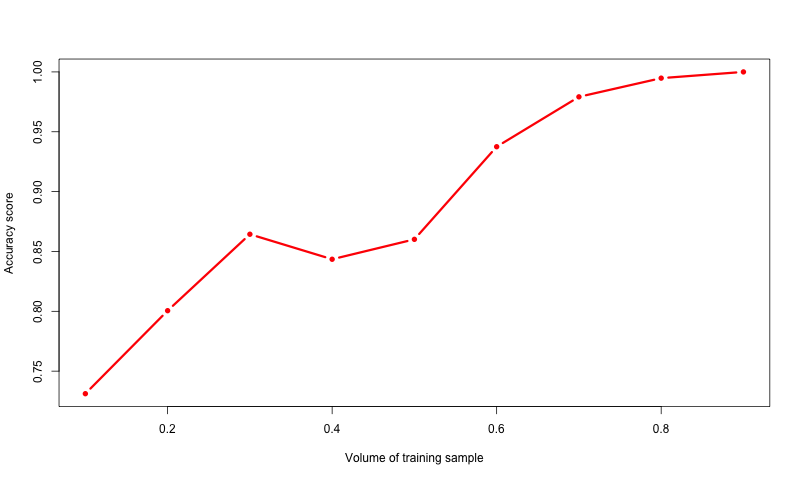
\includegraphics[width = 0.8\linewidth]{data/tic_tac_toe.png}
            \caption{График зависимости для набора <<Крестики-нолики>>}
        \end{figure}
        \vspace{-1cm}
        \begin{figure}[H]
            \centering
            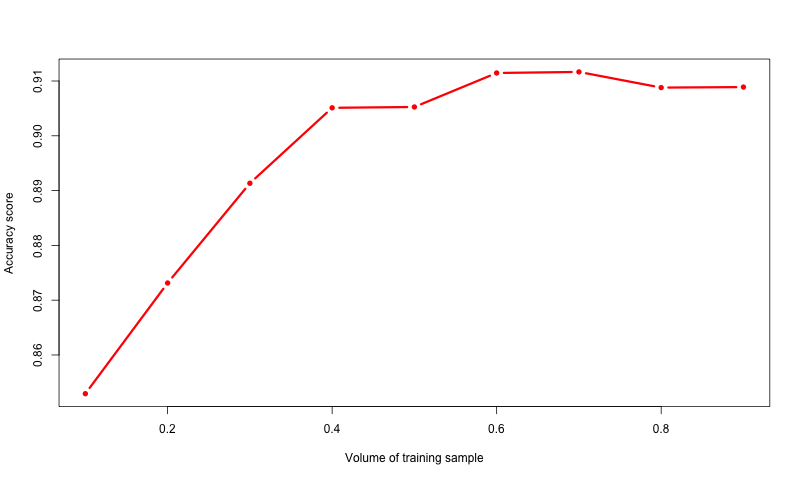
\includegraphics[width = 0.8\linewidth]{data/email.png}
            \caption{График зависимости для набора <<Спам email сообщений>>}
        \end{figure}

    \section{Набор данных <<Glass>>}
        Для того, чтобы исследовать работу алгоритма с предложенным набором данных из него был удален признак <<Id number>> (он не несет информационной нагрузки). Набор данных был разбит на обучающую и тестирующую выборки в соотношении 9:1.

        Обученный алгоритм классифицировал данный в условии задания экземпляр в класс <<5>>.

        Также были проведены исследования того, как значение параметра расстояния Минковского и количество рассматриваемых соседей (k) влияет на точность классификации при использовании разных функций ядра (рис. 3).

        \begin{figure}[H]
            \centering
            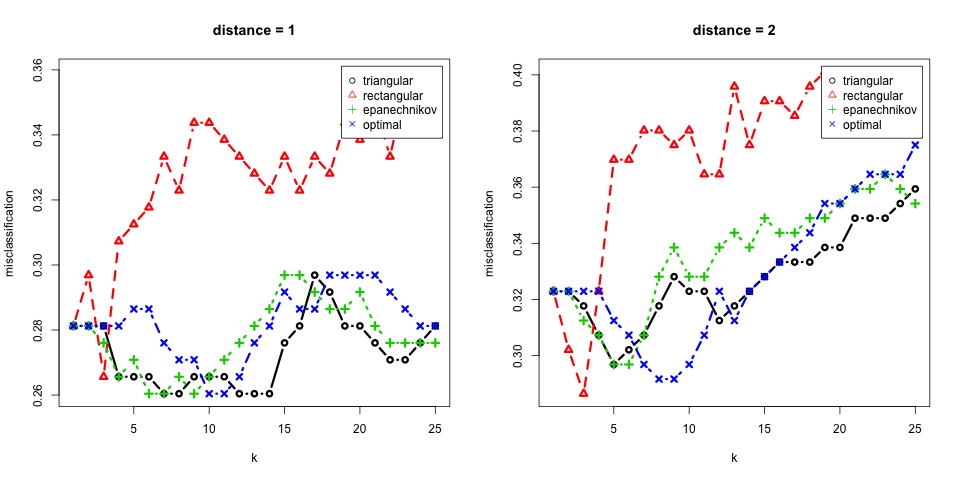
\includegraphics[width = 1.0\linewidth]{data/glass_distance.png}
            \caption{График зависимости для набора <<Glass>>}
        \end{figure}

        Были выяснены оптимальные параметры классификатора для данного набора данных.
        \begin{itemize}
            \item Для параметра расстояния Минковского = 1:
                \begin{itemize}
                    \item Оптимальная функция ядра - треугольная;
                    \item Оптимальное количество соседей - 7.
                \end{itemize}
            \item Для параметра расстояния Минковского = 1:
                \begin{itemize}
                    \item Оптимальная функция ядра - равномерная;
                    \item Оптимальное количество соседей - 3.
                \end{itemize}
        \end{itemize}

        Был проведен анализ того, какой из признаков оказывает наименьшее влияние на определение класса. Для этого был построен график (рис. 4).

        \begin{figure}[H]
            \centering
            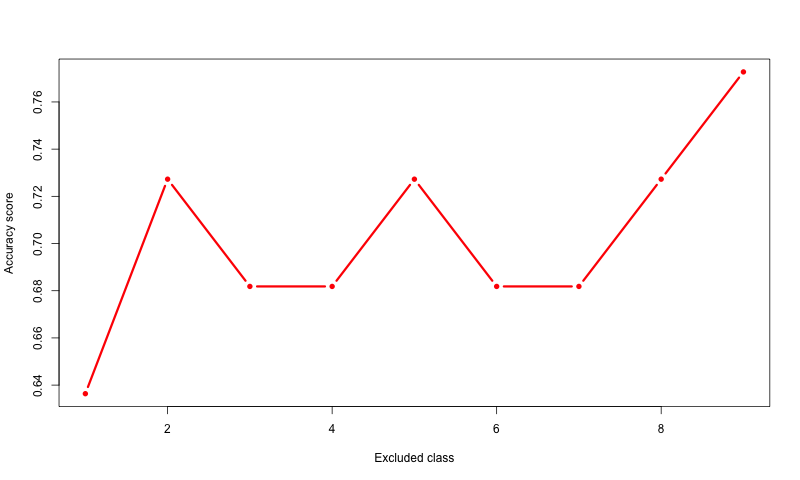
\includegraphics[width = 1.0\linewidth]{data/glass_class_exclude.png}
            \caption{График точности при исключении признаков для набора <<Glass>>}
        \end{figure}

        Говоря напрямую - сложно сказать, какой из признаков оказывает наименьшее влияние, потому что, не смотря на то, что замеры приведены по среднему из 5ти переобучений, возвращаемые значения имеют весьма случайный характер. Однако, чаще всего наименее влияющим оказывался 9ый признак.

    \section{Набор данных <<svmdata4>>}
        Для того, чтобы определить оптимальные значение k и тип функции ядра, был применен метод кросс-валидации. В результате были выявлены следующие значения параметров:
            \begin{itemize}
                \item Функция ядра - <<optimal>>;
                \item Количество соседей - 8.
            \end{itemize}

        Используя такие значения параметров была получена минимальная ошибка 0.03.

        Также были построены графики, визуализирующие исходные данные и результат процесса кросс-валидации (рис. 5).

        \begin{figure}[H]
            \centering
            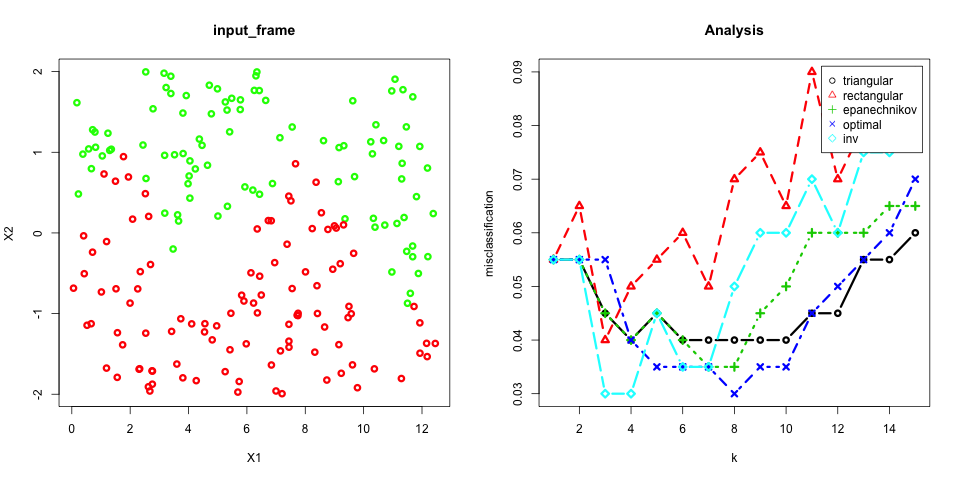
\includegraphics[width = 1.0\linewidth]{data/svmdata.png}
            \caption{Исходные данные и результаты кросс-валидации для набора <<svmdata4>>}
        \end{figure}

    \section{Набор данных <<Titanic>>}

    Был использован метод кросс-валидации для оценки оценки работы данного алгоритма с набором данных <<Titanic>>. На изображении ниже приведены результаты процесса кросс-валидации (рис. 6).

    \begin{figure}[H]
        \centering
        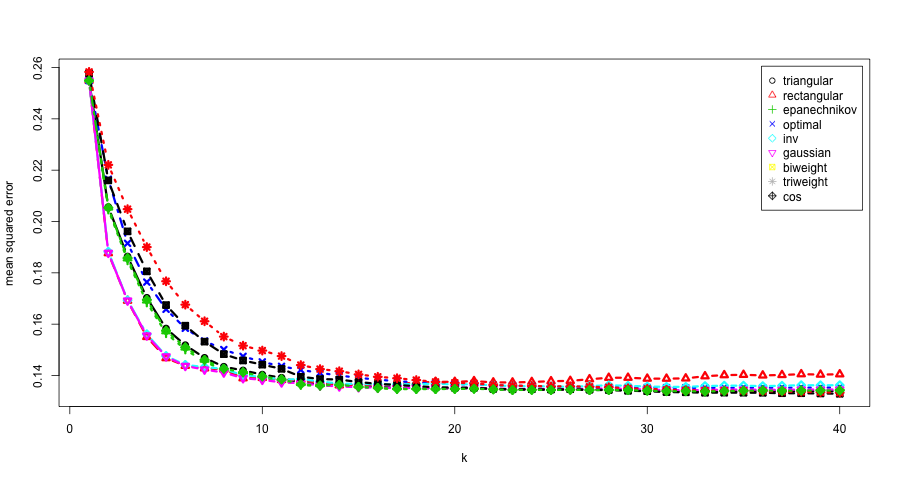
\includegraphics[width = 1.0\linewidth]{data/titanic.png}
        \caption{Результаты кросс-валидации для набора <<svmdata4>>}
    \end{figure}

\end{document}
